\documentclass[11pt]{article}
\usepackage[hmargin={1in},vmargin={1in,1in},foot={.6in}]{geometry}   
\geometry{letterpaper} 
\usepackage{helvet}
\renewcommand{\familydefault}{\sfdefault}    
%\geometry{landscape}          
%\usepackage[parfill]{parskip}
\usepackage{color,graphicx}
%\usepackage{covington}
%\usepackage{xyling}
\usepackage{setspace}
\usepackage{amsmath}
\usepackage{amssymb}
%\usepackage{graphicx,color}
%\usepackage{theorem}
%\usepackage{tabularx}
%\usepackage{subfig}
%\usepackage{vowel}
%\usepackage{mathrsfs}
%\usepackage{varioref}
%\usepackage{textcomp}
%\usepackage{avm}
%\usepackage{textcomp}
%\usepackage{mflogo}
%\usepackage{wasysym}
%\usepackage{pstricks, pst-plot, pst-node, pst-tree, colortab}
%\usepackage{qtree}
 %\usepackage{tree-dvips}
% \usepackage{linguex}
\usepackage{gb4e}
 \usepackage{multirow}
% \usepackage[stable]{footmisc}
% \usepackage{pifont}
%\usepackage{todonotes}
%\usepackage{natbib}
\usepackage{apacite}
%\usepackage[normalem]{ulem}
\usepackage[font=footnotesize,labelfont=bf]{caption}

 %\setlength{\parskip}{.55ex plus 0.1ex}


\usepackage{fancyhdr} % This should be set AFTER setting up the page geometry
\pagestyle{plain} % options: empty , plain , fancy
\lhead{}\chead{}\rhead{}
\renewcommand{\headrulewidth}{.3pt}
\lfoot{}\cfoot{\thepage}\rfoot{}
%\renewcommand{\footrulewidth}{.3pt}
\newcommand{\txtp}{\textipa}
\renewcommand{\rm}{\textrm}
\newcommand{\sem}[1]{\mbox{$[\![$#1$]\!]$}}
\newcommand{\lam}{$\lambda$}
\newcommand{\lan}{$\langle$}
\newcommand{\ran}{$\rangle$}
\newcommand{\type}[1]{\ensuremath{\left \langle #1 \right \rangle }}
\newcommand{\defeq}{$\mathrel{\mathop:}=$ }
\renewcommand{\and}{$\wedge$ }


%\renewcommand{\Extopsep}{2pt}


\newcommand{\bex}{\begin{examples}}
\newcommand{\eex}{\end{examples}}

%bullet points
\newcommand{\bit}{\begin{itemize}}
\newcommand{\eit}{\end{itemize}}

%numbering, non sequential
\newcommand{\ben}{\begin{enumerate}}
\newcommand{\een}{\end{enumerate}}

\renewcommand{\abstractname}{The goal:}


\definecolor{Red}{RGB}{255,0,0}
\newcommand{\red}[1]{\textcolor{Red}{#1}}


\begin{document}

\begin{center}\textbf{When ``all" means not all: nonliteral interpretations of universal quantifiers}\\*[5pt]
\end{center}

\vspace{-11pt}

A great deal of research has examined informativeness-based accounts of scalar implicature such as strengthening ``some" to mean \emph{not all} \shortcite{gazdar1979pragmatics, degen2014processing}; less well studied is the converse effect in which ``all" is relaxed to produce nonliteral interpretations such as \emph{a lot but not all}. For example, ``Bob took all of the credit" means that Bob took more credit than he deserved, and the speaker is upset about it. Recent work has shown that modeling language understanding as reasoning about the speaker's communicative goal can produce hyperbolic interpretations as well as relevant affective subtexts \shortcite{kao2014nonliteral}. Here we describe two experiments that explore people's interpretations of ``all" in different contexts. We then present a computational model that predicts these interpretations by reasoning about informativeness with respect to the speaker's communicative goal.

\textbf{Experiment 1} examines the effect of prior knowledge on interpretations of ``all." In Exp 1a, 60 participants on Mechanical Turk read scenarios in which a character (Ann) brought 10 M\&M�s, cookies, or pies to a party. Participants rated how likely it is that another character (Bob) ate certain amounts of the items. In Exp 1b, 40 participants read scenarios in which Ann said to a friend, ``Bob ate some/all of the M\&M's/cookies/pies!" Participants rated how likely it is that Bob ate certain amounts of items. Results suggest that ``all" is more likely to be interpreted hyperbolically when its literal meaning is increasingly unlikely under the prior distribution ($\beta$=.04, $SE$=.02, $t$=2.45, $p$$<$.05). \textbf{Experiment 2} examines the affect communicated with hyperbolic uses of ``all". In Exp 2a, 40 participants rated how Ann feels given that Bob ate certain amounts of the items; in general, Ann feels more negative the more items Bob eats ($\beta$=.06, $SE$=.003, $t$=20.1, $p$$<$.0001). In Exp 2b, 60 participants rated how Ann feels given that Bob ate certain amounts \emph{and} that she said: ``Bob ate some/all of the M\&M's/cookies/pies!" Even when Bob did not eat all of the items, participants rate Ann as feeling more negative when she says ``all" than when she says ``some" ($\beta$=.31, $SE$=.04, $t$=7.7, $p$$<$.0001, Fig.~2), suggesting that hyperbolic uses of ``all" convey additional affect.

We present an extension to the \textbf{Rational Speech Act model} in which the speaker may want to communicate how many items Bob ate \emph{or} how she feels about it. If Ann wants to communicate negative feelings about Bob, saying ``Bob ate all of the pies" will achieve this effect. Since a pragmatic listener reasons about Ann's communicative goal and knows that it is highly unlikely Bob ate all 10 pies, the listener will infer that Bob ate \emph{some} of the pies, but Ann feels negative about it. Using the priors from Exp. 1a and Exp. 2a, the model produces interpretations that closely match humans' (r=0.91) (Fig. 1). Moreover, the model infers additional affect from hyperbolic uses of ``all" (Fig. 2). Taking together the empirical results and model predictions, we discuss implications on the role of prior knowledge in language processing as well as how it shapes the social and affective information conveyed through nonliteral language.

%In order to recover the intended nonliteral meaning, a pragmatic listener needs to incorporate linguistic information, background knowledge, and the speaker's communicative goal. 
\begin{figure}[h]
\begin{minipage}[b]{.6\textwidth}
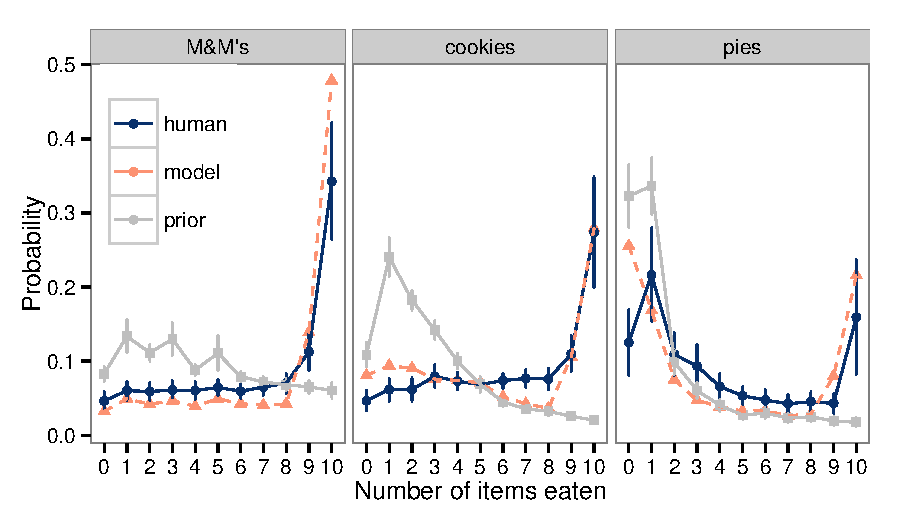
\includegraphics[width=10cm, height=3.7cm]{figure1.pdf}
%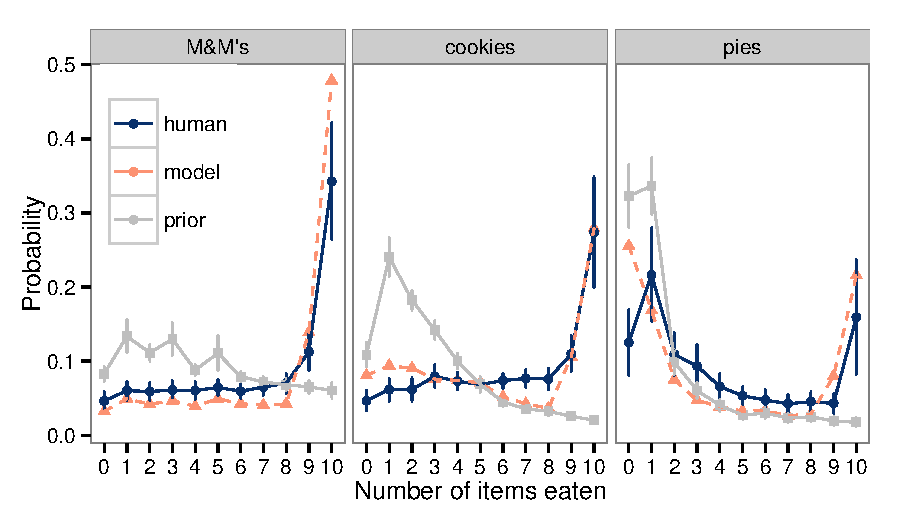
\includegraphics[width=10cm, height=4cm]{figure1.pdf}
\tiny 
\caption{Gray lines (prior) show prior probabilities of Bob eating various amounts given the three food types; blue lines (human) shows participants' interpretations of ``all" for different food types; pink lines (model) shows model predictions.}
\end{minipage}
\begin{minipage}[b]{.4\textwidth}
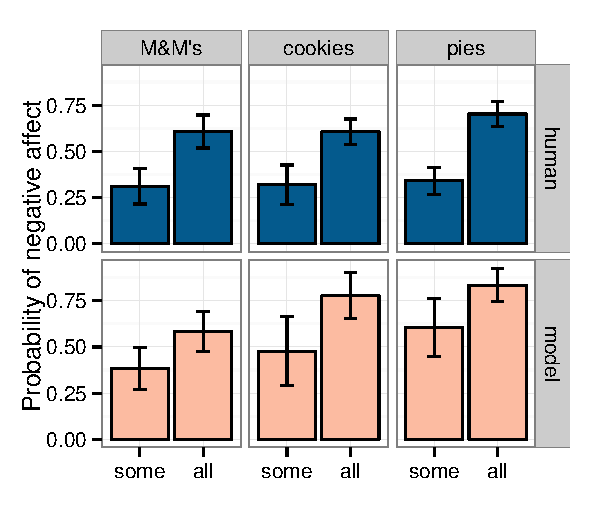
\includegraphics[width=6.5cm, height=3.7cm]{figure2.pdf}
%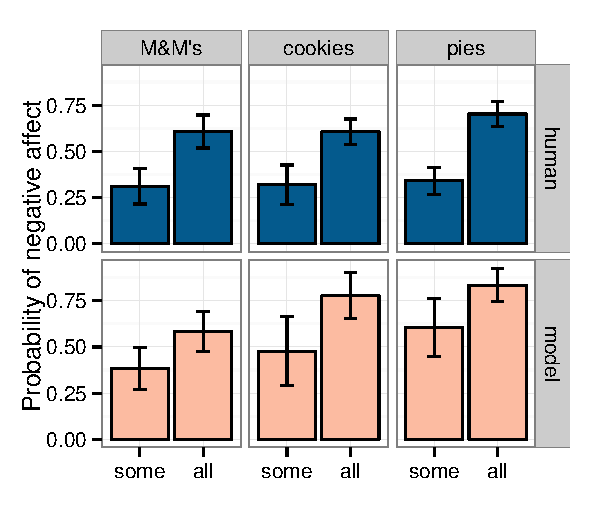
\includegraphics[width=6.5cm, height=4cm]{figure2.pdf}
\caption{Negative affect conveyed in ``some" v.s. ``all." Human data and model both show that hyperbolic uses of ``all" convey more affect than literal uses of ``some."}
\end{minipage}

\label{figure}
\end{figure}

\newpage

\bibliographystyle{chicago}
\bibliography{all.bib}




\end{document}